%!TEX root = ../vernier.tex
\chapter{Related work} \label{sec:related}
Though SoftVis is a comparatively new field to other visualization disciplines, AT\&T Bell Laboratory researchers were already working on visualizing changes in the evolution of software systems in 1992 \cite{seesoft}. Their objective in this particular project was to give project managers an overview of the state of complex systems and provide a tool that allows search for interesting trends and patterns in the development process. As shown in Figure \ref{fig:seesoft}, they have used rectangles to represent files. The height of each rectangle represents the size of the file, and the pixels inside it represent lines of code. These pixel's colors represents the age of the last modification. Blue is used for lines that haven't been modified in a long time and red is used for recent changes.

\begin{figure}[H]
	\centering
	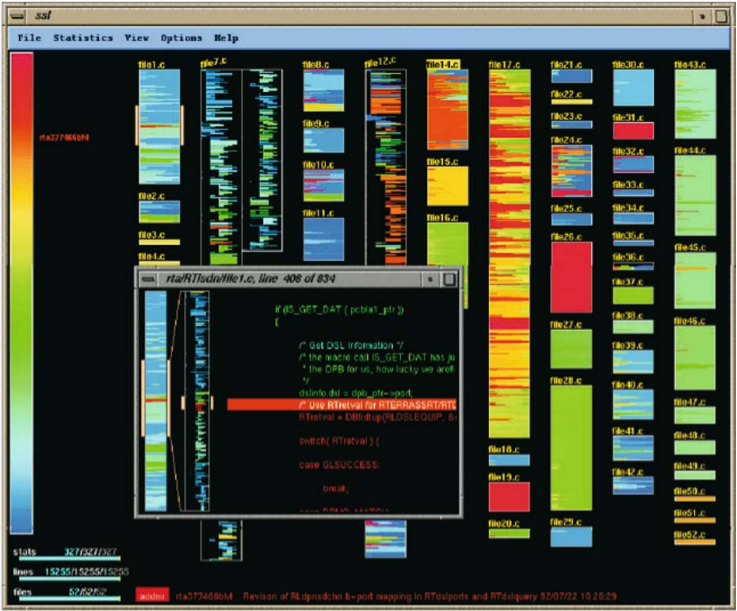
\includegraphics[width=1.0\textwidth]{figures/seesoft.png}
	\caption{SeeSoft circa 1992}
	\label{fig:seesoft}
\end{figure}

According to Ian \citet{Sommerville:2004:SE:983346}, 90\% of the cost of software development is linked to maintenance tasks. SolidSX \cite{ref:solid}, CVSscan \cite{voinea2005}, and CVSgrab \cite{VisSymEuroVis06} are tools that use evolution visualization techniques to help developers better execute these tasks. They use linked views (e.g. treemaps, table lenses, and hierarchical edge bundles) to aid correlation between source code structure and relationships with its evolution in time, hopefully aiding in this expensive process.

\begin{figure}
 \centering
 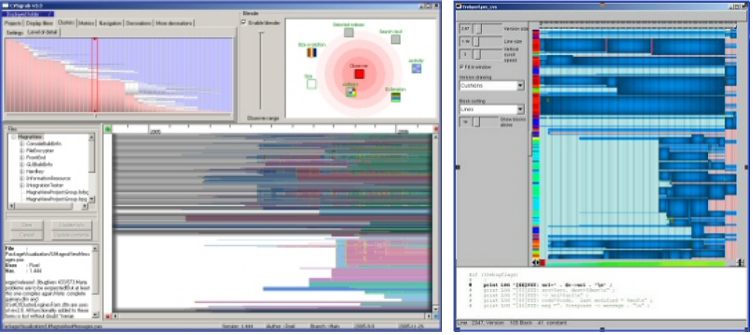
\includegraphics[width=1.0\textwidth]{figures/cvs.png}
 \caption{CVSgrab on the left and CVSscan on the right}
 \legend{Source: \cite{voinea2005} and \cite{VisSymEuroVis06}}
 \label{fig:cvs}
\end{figure}

\begin{figure}
	\centering
	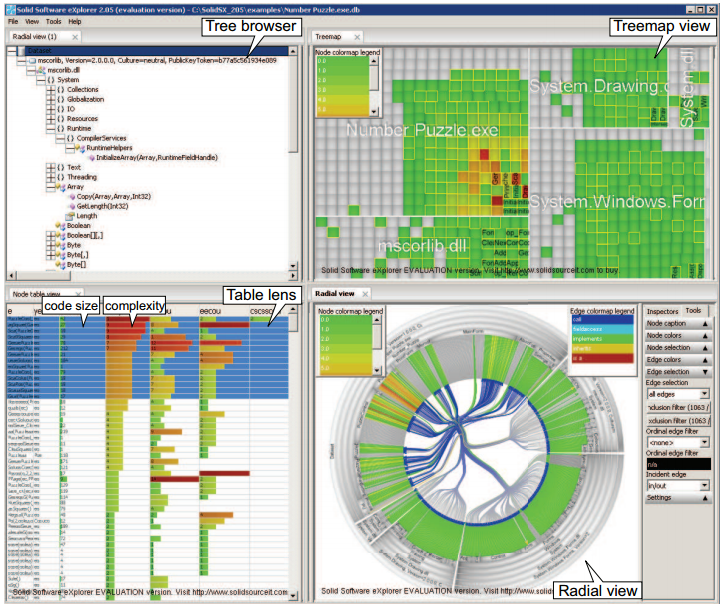
\includegraphics[width=0.8\textwidth]{figures/solidsx.png}
	\caption{SolidSX views}
	\legend{Source: \cite{ref:solid}}
	\label{fig:solidsx}
\end{figure}

In a more recent approach \citet{ref:silva2} used extracted quality metrics from software repositories in a multidimensional visualization context, proposing dynamic maps that show the evolution of the similarity of entities across revisions. We have taken part in this project and in this work, we attempt to extend our understanding of the problem.

\begin{figure}
	\centering
	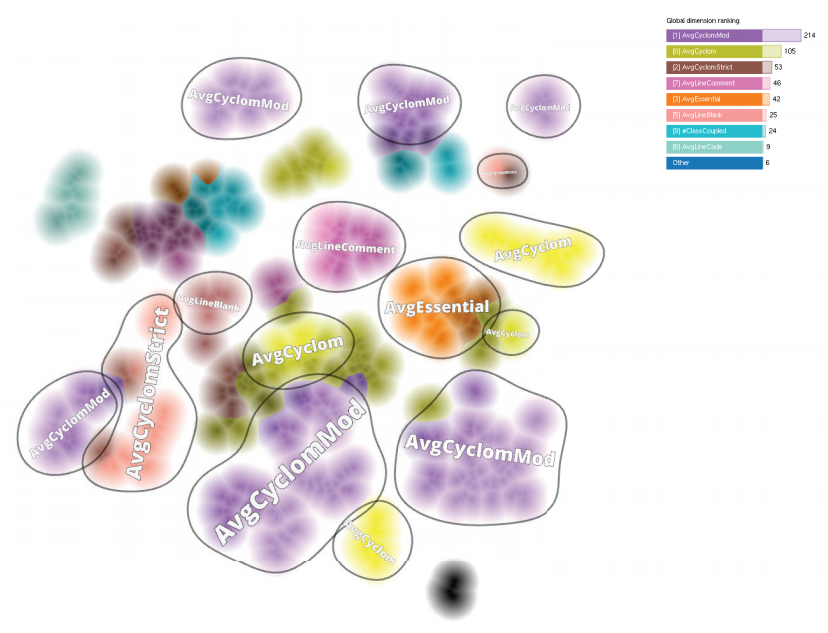
\includegraphics[width=0.8\textwidth]{figures/mem.png}
	\caption{Projections being used to display class similarity, labeling the attribute that most strongly collaborated in bring these entities together.}
	\legend{Source: \cite{ref:silva2}}
	\label{fig:mem}
\end{figure}
